\documentclass{article}
\usepackage{polski}
\usepackage[utf8]{inputenc}
\usepackage{float}
\usepackage{graphicx}
\usepackage{caption}
\usepackage{subcaption}
\usepackage{ragged2e}
\usepackage{amsmath}
\usepackage{amssymb}
\usepackage{amsfonts}
\usepackage{blindtext}
\usepackage{hyperref}
\usepackage{listings}
\usepackage{booktabs}
\usepackage{siunitx}
\usepackage{multicol}
\usepackage{fancyvrb}
\usepackage[linesnumbered,ruled,vlined]{algorithm2e}

\begin{document}

\AddToHook{cmd/section/before}{\clearpage}

\section*{Zadanie 1}
Naszym celem w tym zadaniu jest zaimplementowanie funkcji, która będzie liczyć
ilorazy różnicowe.
Jako parametry nasza funkcja bierze dwa wektory, konceptualnie przedstawiają
one pary punktów $(x_i, f(x_i))$. Dzięki nim możemy wyznaczyć ilorazy różnicowe.
Robimy to w następujący sposób:
\[
\begin{array}[t]{ccccc}
f[x_0] & & & & \\
& f[x_0, x_1] & & & \\
f[x_1] & & f[x_0, x_1, x_2] & & \\
& f[x_1, x_2] & & f[x_0, x_1, x_2, x_3] & \\
f[x_2] & & f[x_1, x_2, x_3] & & \\
& f[x_2, x_3] & & & \\
f[x_3] & & & & \\
\end{array}
\]
konceptualnie nasz wynikowy wektor będzie się "zmniejszał".
To znaczy, pamięciowo będzie zajmował tyle samo miejsca, ale
wartości używanych w obliczeniach będzie coraz mniej. Do wektora
wynikowego będziemy pushować $f[1]$ co iterację algorytmu.
\begin{algorithm}[h]
    \SetAlgoLined
    \KwResult{Ilorazy różnicowe \(f[x_0, x_1, \dots, x_i]\)}
    \KwIn{\(x\), wektor punktów \(x_i\)}
    \KwIn{\(f\), wektor wartości \(f(x_i)\) w punktach \(x_i\)}
    
    \SetKwFunction{FMain}{ilorazyRoznicowe}
    \SetKwProg{Fn}{Function}{:}{}
    \Fn{\FMain{\(x\), \(f\)}}{
        \(n \leftarrow \) len\((x)\);\\
        \(ret \leftarrow \) \([f[1]]\);\\
        \For{\(i \leftarrow 1\) \KwTo \(n-1\)}{
            \For{\(j \leftarrow 1\) \KwTo \(n-i\)}{
                \(f[j] \leftarrow \frac{f[j + 1] - f[j]}{x[i + j] - x[j]}\)\;
            }
            Append \(f[1]\) to \(ret\)\;
        }
        \KwRet \(ret\)\;
    }
\end{algorithm}
\subsection*{Złożoność}
Złożoność czasowa naszego algorytmu jest rzędu $O(n^2)$, gdzie $n$ to rozmiar wektora $x$.
Natomiast pamięciowa jest rzędu $O(n)$.

\section*{Zadanie 2}
W tym zadaniu mamy zaimplementować funkcję, która będzie liczyć wartość
wielomianu interpolacyjnego w punkcie $t$. Na wykładzie mieliśmy podany wzór:
\[
p_n(x) = \sum_{k=0}^{n} c_k q_k(x) = \sum_{k=0}^{n} f[x_0, x_1, \ldots, x_k] \prod_{j=0}^{k-1} (x - x_j).
\]
Łatwo jednak zauważyć, że jego złożoność jest rzędu $O(n^2)$, ponieważ
w każdej iteracji pętli musimy wykonać $k$ mnożeń. Przy pomocy
uogólnionego algorytmu Hornera możemy zredukować złożoność do $O(n)$.
\begin{algorithm}[h]
    \SetAlgoLined
    \KwResult{Wartość wielomianu interpolacyjnego w punkcie \(t\)}
    \KwIn{\(x\), wektor punktów \(x_i\)}
    \KwIn{\(fx\), wetkor ilorazów różnicowych \(f[x_0, x_1, \dots, x_i]\)}
    \KwIn{\(t\), punkt w którym chcemy policzyć wartość wielomianu}
    
    \SetKwFunction{FMain}{warNewton}
    \SetKwProg{Fn}{Function}{:}{}
    \Fn{\FMain{\(x\), \(fx\), \(t\)}}{
        \(nt \leftarrow 0\)\;
        \For{\(i \leftarrow \) length of \(x\) \KwTo \(1\)}{
            \(nt \leftarrow fx[i] + nt * (t - x[i])\)\;
        }
        \KwRet \(nt\)\;
    }
\end{algorithm}

\section*{Zadanie 3}
W tym zadaniu mamy zaimplementować funkcję, która będzie liczyć
współczynniki wielomianu w postaci naturalnej korzystając
z tego, że znamy wartości współczynników w postaci Newtona.
Konkretnie chcemy obliczyć wektor współczynników $a_i$ takich że:
\[
p_n(x) = \sum_{i=0}^{n} c_i \prod_{j=0}^{i-1} (x - x_j) = \sum_{i=0}^{n} a_i x^i.
\]
Widzimy, że nasz wielomian jest dany wzorem:
\[
p_n(x) = c_0 + c_1(x - x_0) + c_2(x - x_0)(x - x_1) + \cdots + c_n(x - x_0)(x - x_1)\dots(x - x_{n-1}).
\]
Przyjrzyjmy się więc temu jak możemy wyciągnąć poszczególne współczynniki.
Przy $x^n$ mamy tylko jeden czynnik, więc $a_n = c_n$. Ale przy $x^{n-1}$
mamy $c_{n-1}$ ze składnika zawierającego $x^{n-1}$ oraz $n \choose 1$
składników ze składnika zawierającego $x^n$,
$-c_{n}x_{i}$ dla $i \in \{0, 1, \dots, n-1\}$. Z tego względu złożoność
byłaby bardzo wysoka, gdybyśmy chcieli obliczyć współczynniki tym sposobem.
Zauważmy jednak, że możemy to zrobić w czasie kwadratowym, odejmując
$a_{j+1} \cdot x_i$ gdzie $i$ to stopień $x^i$, który obecnie rozwijamy,
a $j$ to indeks w naszym wektorze $a$ o wartościach $j \in \{i, i+1, \dots, n-1\}$,
od którego odejmujemy nasz odjemnik.

\begin{algorithm}[H]
    \SetAlgoLined
    \KwResult{Współczynniki wielomianu w postaci naturalnej}
    \KwIn{\(x\), wektor punktów \(x_i\)}
    \KwIn{\(fx\), wektor ilorazów różnicowych \(f[x_0, x_1, \dots, x_i]\)}
    
    \SetKwFunction{FMain}{naturalna}
    \SetKwProg{Fn}{Function}{:}{}
    \Fn{\FMain{\(x\), \(fx\)}}{
        \(n \leftarrow \) len(\(x\))\;
        \(a \leftarrow \) zeros\((n)\)\;
        \(a[n] \leftarrow fx[n]\)\;
    
        \For{\(i \leftarrow \) $n$ down to \(1\)}{
            \For{\(j \leftarrow i\) to \(n-1\)}{
                \(a[j] \leftarrow a[j] - a[j+1] \times x[i]\)\;
            }
            \(a[i] \leftarrow a[i] + fx[i]\)\;
        }
        \KwRet \(a\)\;
    }
\end{algorithm}

\subsection*{Złożoność}
Złożoność czasowa naszego algorytmu jest rzędu $O(n^2)$, gdzie $n$ to rozmiar wektora $x$.
Natomiast pamięciowa jest rzędu $O(n)$.

\section*{Zadanie 4}
W tym zadaniu mamy zaimplementować funkcję, która wizualizuje
funkcję $f$ oraz jej interpolację $w$ na przedziale $[a, b]$.

Przedział dzielimy na $n+1$ równoodległych punktów,
$\text{points\_f}_i = a+i(\frac{b-a}{n})$ gdzie $n$ to stopień
wielomianu interpolacyjnego. Następnie liczymy wartości funkcji $f$ w tych
punktach. Na podstawie tych wartości liczymy ilorazy różnicowe.

Ustalamy, że między dwoma kolejnymi punktami będziemy rysować
100 punktów. Dzięki temu nasz wykres będzie wyglądał na gładki.
Następnie liczymy wartości $f$ oraz $w$ (przy użyciu wcześniej
zaimplementowanej funkcji warNewton) w tych punktach
i rysujemy je na przedziale $[a,b]$ przy pomocy Julia Plots.
\begin{algorithm}[h]
    \SetAlgoLined
    \KwIn{\(f\), funkcja, której interpolację chcemy narysować}
    \KwIn{\(a\), lewy koniec przedziału}
    \KwIn{\(b\), prawy koniec przedziału}
    \KwIn{\(n\), stopień wielomianu interpolacyjnego}
    \KwOut{Wykres funkcji \(f\) oraz jej interpolacji \(w\)}
    
    \SetKwFunction{FMain}{rysujNnfx}
    \SetKwProg{Fn}{Function}{:}{}
    \Fn{\FMain{\(f\), \(a\), \(b\), \(n\)}}{
        \(h \leftarrow \frac{b - a}{n}\)\;
        \(points\_f \leftarrow \) wektor \([a + i * h\) for \(i\) in \(0\) to \(n]\)\;
        \(values\_f \leftarrow \) wektor \([f(x)\) for \(x\) in \(points\_f]\)\;
    
        \(fx \leftarrow \) call \(ilorazyRoznicowe(points\_f, values\_f)\)\;
    
        \(points\_num \leftarrow 100 * n + 1\)\;
        \(delta \leftarrow \frac{b - a}{points\_num - 1}\)\;
    
        \(x\_values \leftarrow \) wektor \([a + i * delta\) for \(i\) in \(0\) to \(points\_num-1]\)\;
        \(y\_values \leftarrow \) wektor \([f(x)\) for \(x\) in \(x\_values]\)\;
        \(w\_values \leftarrow \) wektor \([warNewton(points\_f, fx, x)\) for \(x\) in \(x\_values]\)\;

        \(plot(f(x))\)\;
        \(plot(warNewton(points\_f, fx, x))\)\;
    }
\end{algorithm}

\section*{Zadanie 5}
W tym zadaniu mamy zwizualizować przy pomocy funkcji z zadania 4
następujące funkcje:
\begin{gather*}
    n \in \{5, 10, 15\},\\
    f(x) = e^x \text{ dla } [a, b] = [0, 1],\\
    f(x) = x^2 \sin(x) \text{ dla } [a, b] = [-1, 1]\\
\end{gather*}

\begin{figure}[H]
    \centering
    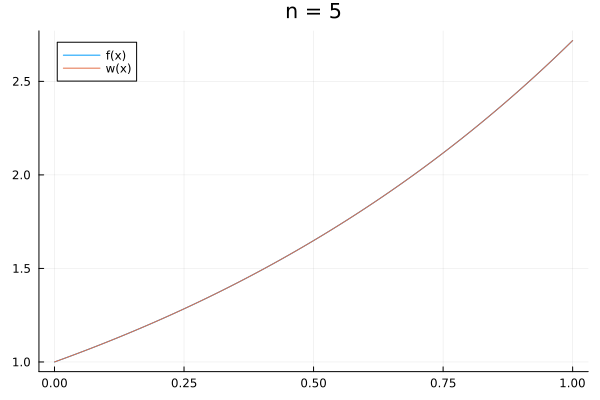
\includegraphics[width=0.9\textwidth]{../plots/ex4_1_n5.png}
    \caption{Wykresy porównujące funkcję $f(x) = e^x$ oraz jej interpolację $w(x)$ na przedziale $[-1, 1]$ i $n=5$.}
\end{figure}
\begin{figure}[H]
    \centering
    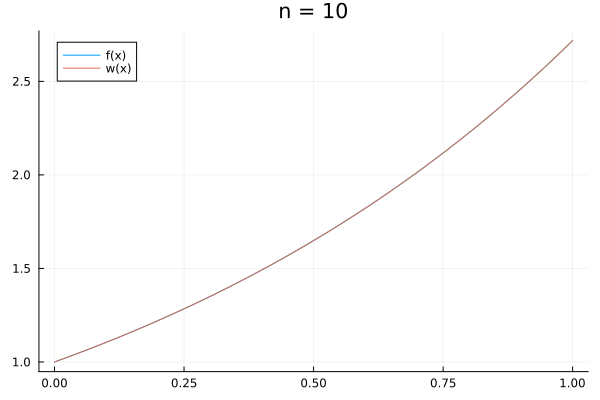
\includegraphics[width=0.9\textwidth]{../plots/ex4_1_n10.png}
    \caption{Wykresy porównujące funkcję $f(x) = e^x$ oraz jej interpolację $w(x)$ na przedziale $[-1, 1]$ i $n=10$.}
\end{figure}
\begin{figure}[H]
    \centering
    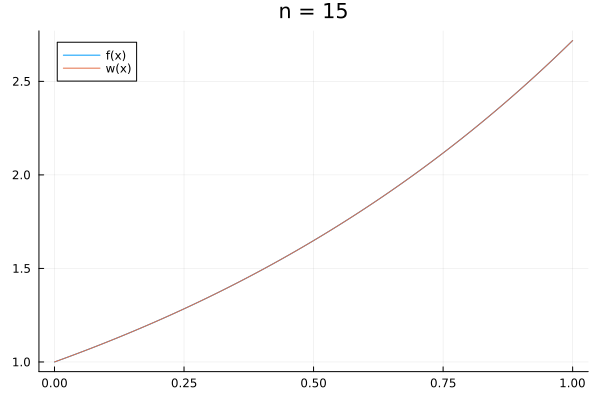
\includegraphics[width=0.9\textwidth]{../plots/ex4_1_n15.png}
    \caption{Wykresy porównujące funkcję $f(x) = e^x$ oraz jej interpolację $w(x)$ na przedziale $[-1, 1]$ i $n=15$.}
\end{figure}
\begin{figure}[H]
    \centering
    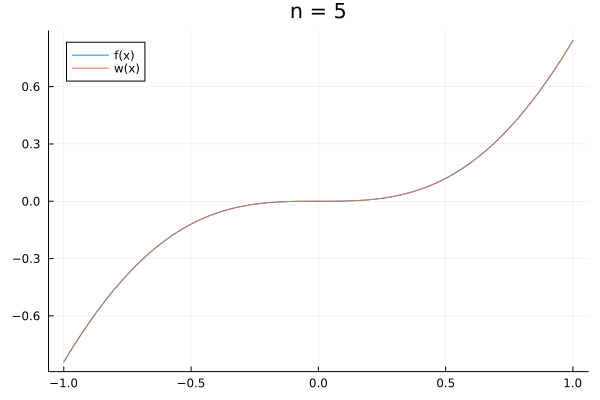
\includegraphics[width=0.9\textwidth]{../plots/ex4_2_n5.png}
    \caption{Wykresy porównujące funkcję $f(x) = x^2\sin(x)$ oraz jej interpolację $w(x)$ na przedziale $[-1, 1]$ i $n=5$.}
\end{figure}
\begin{figure}[H]
    \centering
    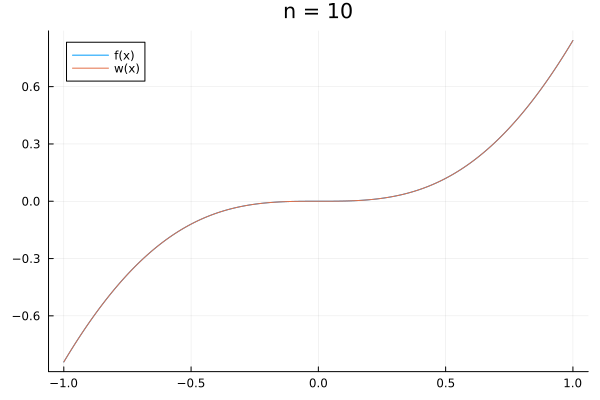
\includegraphics[width=0.9\textwidth]{../plots/ex4_2_n10.png}
    \caption{Wykresy porównujące funkcję $f(x) = x^2\sin(x)$ oraz jej interpolację $w(x)$ na przedziale $[-1, 1]$ i $n=10$.}
\end{figure}
\begin{figure}[H]
    \centering
    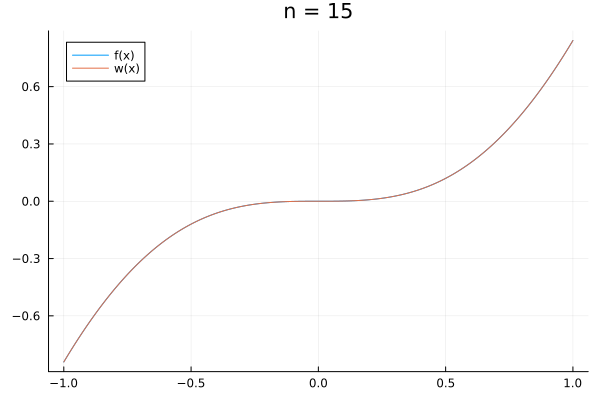
\includegraphics[width=0.9\textwidth]{../plots/ex4_2_n15.png}
    \caption{Wykresy porównujące funkcję $f(x) = x^2\sin(x)$ oraz jej interpolację $w(x)$ na przedziale $[-1, 1]$ i $n=15$.}
\end{figure}


\subsection*{Interpretacja wyników}
Na wykresach widać, że już dla wielomianu stopnia 5 wykresy funkcji $f$ oraz $w$
się pokrywają. Jest to zgodne z intuicją, ponieważ obie te funkcje są gładkie i
na danym przedziale mają mniej punktów przegięcia niż 5.



\section*{Zadanie 6}
W tym zadaniu mamy zwizualizować przy pomocy funkcji z zadania 4
następujące funkcje:
\begin{gather*}
    n \in \{5, 10, 15\},\\
    f(x) = |x| \text{ dla } [a, b] = [-1, 1],\\
    f(x) = \frac{1}{1+x^2} \text{ dla } [a, b] = [-5, 5]\\
\end{gather*}

\begin{figure}[H]
    \centering
    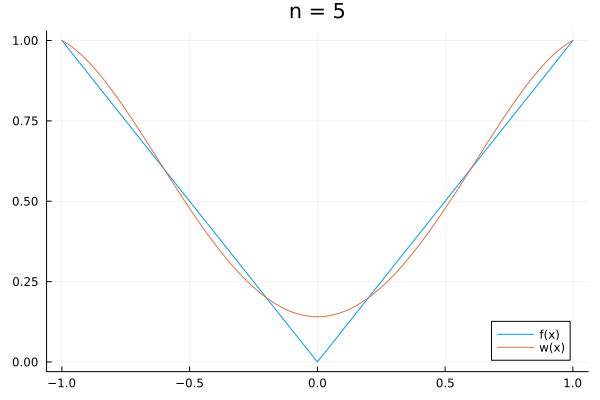
\includegraphics[width=0.9\textwidth]{../plots/ex5_1_n5.png}
    \caption{Wykresy porównujące funkcję $f(x) = |x|$ oraz jej interpolację $w(x)$ na przedziale $[-1, 1]$ i $n=5$.}
\end{figure}
\begin{figure}[H]
    \centering
    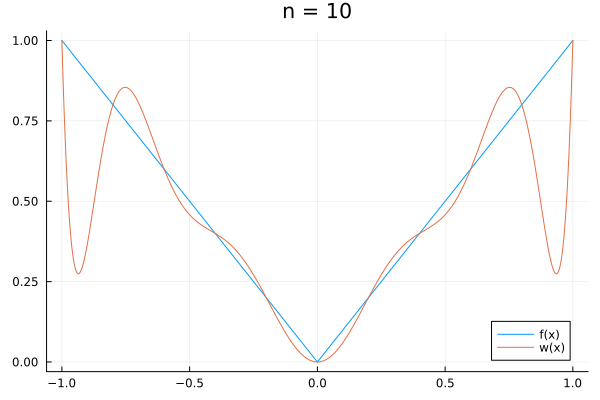
\includegraphics[width=0.9\textwidth]{../plots/ex5_1_n10.png}
    \caption{Wykresy porównujące funkcję $f(x) = |x|$ oraz jej interpolację $w(x)$ na przedziale $[-1, 1]$ i $n=10$.}
\end{figure}
\begin{figure}[H]
    \centering
    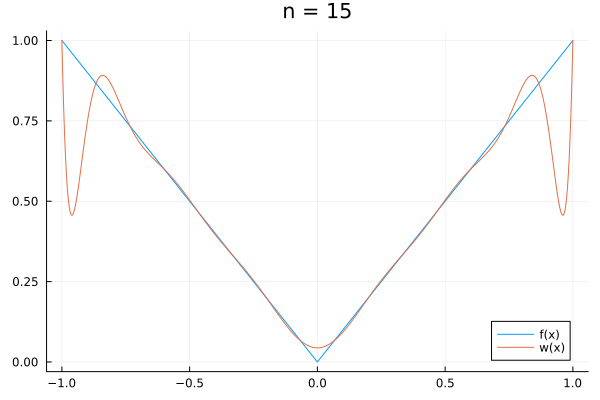
\includegraphics[width=0.9\textwidth]{../plots/ex5_1_n15.png}
    \caption{Wykresy porównujące funkcję $f(x) = |x|$ oraz jej interpolację $w(x)$ na przedziale $[-1, 1]$ i $n=15$.}
\end{figure}
\begin{figure}[H]
    \centering
    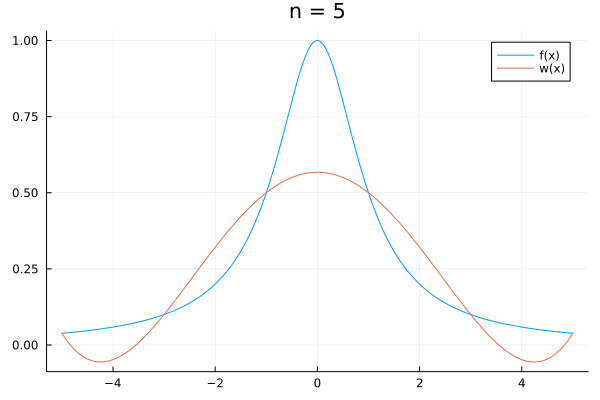
\includegraphics[width=0.9\textwidth]{../plots/ex5_2_n5.png}
    \caption{Wykresy porównujące funkcję $f(x) = \frac{1}{1+x^2}$ oraz jej interpolację $w(x)$ na przedziale $[-5, 5]$ i $n=5$.}
\end{figure}
\begin{figure}[H]
    \centering
    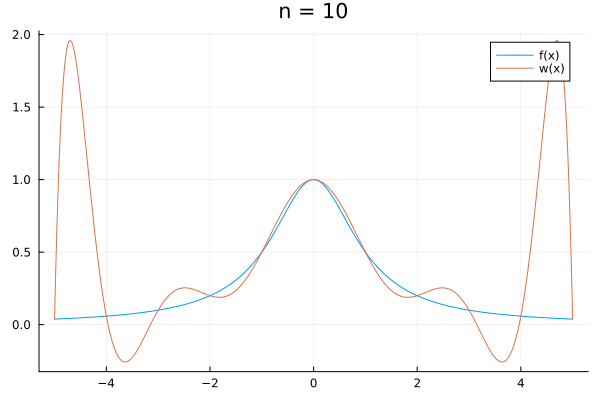
\includegraphics[width=0.9\textwidth]{../plots/ex5_2_n10.png}
    \caption{Wykresy porównujące funkcję $f(x) = \frac{1}{1+x^2}$ oraz jej interpolację $w(x)$ na przedziale $[-5, 5]$ i $n=10$.}
\end{figure}
\begin{figure}[H]
    \centering
    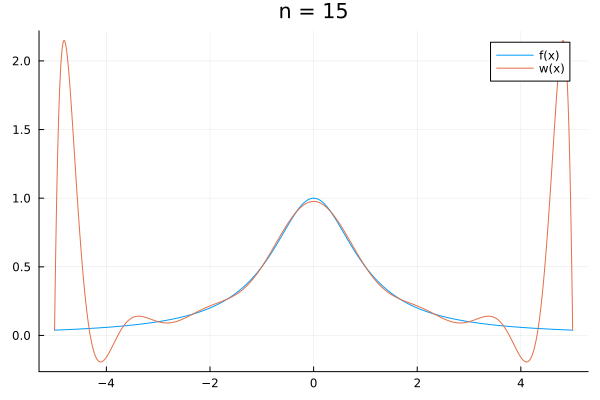
\includegraphics[width=0.9\textwidth]{../plots/ex5_2_n15.png}
    \caption{Wykresy porównujące funkcję $f(x) = \frac{1}{1+x^2}$ oraz jej interpolację $w(x)$ na przedziale $[-5, 5]$ i $n=15$.}
\end{figure}

\subsection*{Interpretacja wyników}
Tym razem funkcje $f$ oraz $w$ nie pokrywają się na naszych wykresach.

W przypadku $f(x) = |x|$ jednym z problemów jest to, że nie jest ona
różniczkowalna w punkcie $x=0$. Intuicyjcnie, wielomiany są gładkie, a tymczasem
funkcja $f$ ma w $x=0$ punkt przegięcia o kącie prostym. Możemy pomyśleć, że odpowiednio
wysokie zwiększenie stopnia wielomianu zredukuje ten problem. Widzimy jednak, że
powiększanie $n$ zniekształca wykres na krańcach przedziału.

Funcja $f(x) = \frac{1}{1+x^2}$ jest gładka, ale tym razem podobnie jak przy poprzedniej
funkcji, zwiększanie $n$ zniekształca wykres na krańcach przedziału. Jest to przykład
efektu Rungego.

\subsection*{Efekt Rungego}
Zniekształcanie funkcji na krańcach przedziału przy zwiększaniu stopnia wielomianu
nazywamy efektem Rungego. Jest to zjawisko, które występuje przy interpolacji
funkcji za pomocą wielomianów wysokiego stopnia na równoodległych węzłach,
czyli to co robimy u nas.

Na wykładzie mieliśmy podane twierdzenie o błędzie interpolacji:
\[
f(x) - p(x) = \frac{1}{(n + 1)!} f^{(n+1)}(\xi_{x}) \prod_{i=0}^{n} (x - x_i).
\]
Z tego równania widać, że im więcej punktów interpolacji, tym mniejszy jest iloczyn
$\prod_{i=0}^{n} (x - x_i)$. Oznacza to więc, że gdy nta pochodna funkcji $f$ w danym
punkcie jest znacznie większa od $(n+1)!$ to wahania błędu w jego sąsiedztwie będą
również duże.

\subsubsection*{Jak zapobiec efektowi Rungego?}
Jednym ze sposobów jest skorzystanie z innego rozkładu punktów. Konkretnie chcemy
mieć więcej punktów na krańcach przedziału. Przykładem takiego rozkładu jest
rozkład Czebyszewa. Gdy tak jak tutaj korzystamy z równoodległych węzłów, to
możemy na nich zastosować algorytm S-Runge, który mapuje nasze węzły na
takie z rozkładem Czebyszewa.

Kolejnym sposobem jest użycie funkcji sklejanych z kawałkami wielomianowymi.

\end{document}